\documentclass[11pt]{beamer}
\usepackage{tikz}
\usetikzlibrary{decorations.pathreplacing}
\usepackage{verbatim}
\usepackage{tkz-berge}
\usepackage{algpseudocode}
\usepackage{tikz}
\usetikzlibrary{calc,fit}
\usetheme{Frankfurt}

\title[Counting and Sampling Triangles from a Graph Stream] % (optional, only for long titles)
{Counting and Sampling Triangles from a Graph Stream}
\subtitle{A. Pavan, Kanat Tangwongsan, Srikanta Tirthapura, Kun-Lung Wu\\2013, VLDB Conference}
\author[] % (optional, for multiple authors)
{Marten Heidemeyer}
\date[\today] % (optional)
{Presentation for CMPT 843 Class}
\subject{Computer Science}


\begin{document}
\frame{\titlepage}
\begin{frame}
\frametitle{Outline}
\tableofcontents[]
\end{frame}
\section{Motivation}
\begin{frame}
\frametitle{Motivation}
\begin{itemize}
\item Triangle Counting is important in:
\begin{itemize}
\item social networks
\item spam and fraud detection
\item link classification and recommendation
\end{itemize}
\item Why use a streaming algorithm?
\begin{itemize}
\item real-time processing of live data
\item analysis of \textbf{large} disk-resident graph data
\end{itemize}
\end{itemize}
\end{frame}

\section{Neighborhood Sampling}
\begin{frame}

\frametitle{The Adjacency Stream Model}
\framesubtitle{1}
\begin{center}
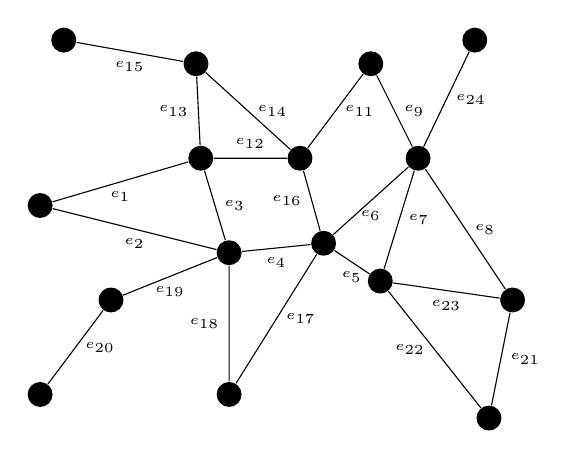
\begin{tikzpicture}[scale=0.6]
\tikzstyle{vertex}=[circle,fill=black,minimum size=9pt,inner sep=0pt]
\foreach \name/\point in {
	1/{-1,-1},
	2/{-1,3},
	3/{2.4,4},
	4/{5,2.2},
	5/{2.3,6},
	6/{6.2,1.4},
	7/{4.5,4},
	8/{-0.5,6.5},
	9/{3,-1},
	11/{3,2},
	10/{0.5,1},
	12/{6,6},
	13/{7,4},
	14/{9,1},
	15/{8.5,-1.5},
	16/{8.2,6.5}}
 	\node[vertex] (\name) at (\point) {};
\draw (2) -- (3) node[draw=none,fill=none,midway,below,font=\tiny] {$e_1$};
\draw (2) -- (11) node[draw=none,fill=none,midway,below,font=\tiny] {$e_2$};
\draw (3) -- (11) node[draw=none,fill=none,midway,right,font=\tiny] {$e_3$};
\draw (11) -- (4)node[draw=none,fill=none,midway,below,font=\tiny] {$e_4$};
\draw (4) -- (6)node[draw=none,fill=none,midway,below,font=\tiny] {$e_5$};
\draw (4) -- (13)node[draw=none,fill=none,midway,below,font=\tiny] {$e_6$};
\draw (6) -- (13)node[draw=none,fill=none,midway,right,font=\tiny] {$e_7$};
\draw (13) -- (14)node[draw=none,fill=none,midway,right,font=\tiny] {$e_8$};
\draw (13) -- (12)node[draw=none,fill=none,midway,right,font=\tiny] {$e_9$};
\draw (12) -- (7)node[draw=none,fill=none,midway,right,font=\tiny] {$e_{11}$};
\draw (7) -- (3)node[draw=none,fill=none,midway,above,font=\tiny] {$e_{12}$};
\draw (3) -- (5)node[draw=none,fill=none,midway,left,font=\tiny] {$e_{13}$};
\draw (5) -- (7)node[draw=none,fill=none,midway,right,font=\tiny] {$e_{14}$};
\draw (5) -- (8)node[draw=none,fill=none,midway,below,font=\tiny] {$e_{15}$};
\draw (7) -- (4)node[draw=none,fill=none,midway,left,font=\tiny] {$e_{16}$};
\draw (9) -- (4)node[draw=none,fill=none,midway,right,font=\tiny] {$e_{17}$};
\draw (11) -- (9)node[draw=none,fill=none,midway,left,font=\tiny] {$e_{18}$};
\draw (11) -- (10)node[draw=none,fill=none,midway,below,font=\tiny] {$e_{19}$};
\draw (10) -- (1)node[draw=none,fill=none,midway,right,font=\tiny] {$e_{20}$};
\draw (14) -- (15)node[draw=none,fill=none,midway,right,font=\tiny] {$e_{21}$};
\draw (6) -- (15)node[draw=none,fill=none,midway,left,font=\tiny] {$e_{22}$};
\draw (14) -- (6)node[draw=none,fill=none,midway,below,font=\tiny] {$e_{23}$};
\draw (13) -- (16)node[draw=none,fill=none,midway,right,font=\tiny] {$e_{24}$};
\end{tikzpicture}
\end{center}
\begin{center}
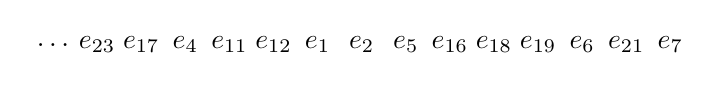
\begin{tikzpicture}[scale=0.8]
\tikzstyle{recti}=[rectangle,draw=red,thick,minimum width=0.5cm,minimum height=0.4cm]
\tikzstyle{stream}=[rectangle]
\node [stream] at (-0.7,0){$\dots$};
\node [stream] at (0,0) {$e_{23}$};
\node [stream] at (0.7,0) {$e_{17}$};
\node [stream] at (1.4,0) {$e_{4}$};
\node [stream] at (2.1,0) {$e_{11}$};
\node [stream] at (2.8,0) {$e_{12}$};
\node [stream] at (3.5,0) {$e_{1}$};
\node [stream] at (4.2,0) {$e_{2}$};
\node [stream] at (4.9,0) {$e_{5}$};
\node [stream] at (5.6,0) {$e_{16}$};
\node [stream] at (6.3,0) {$e_{18}$};
\node [stream] at (7.0,0) {$e_{19}$};
\node [stream] at (7.7,0) {$e_{6}$};
\node [stream] at (8.4,0) {$e_{21}$};
\node [stream] at (9.1,0) {$e_{7}$};
\end{tikzpicture}
\end{center}
\end{frame}
\begin{frame}


\frametitle{The Adjacency Stream Model}
\framesubtitle{2}
\begin{center}
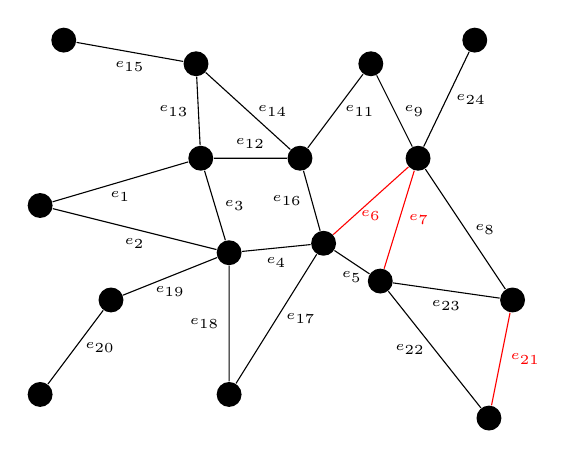
\begin{tikzpicture}[scale=0.6]
\tikzstyle{vertex}=[circle,fill=black,minimum size=9pt,inner sep=0pt]
\foreach \name/\point in {
	1/{-1,-1},
	2/{-1,3},
	3/{2.4,4},
	4/{5,2.2},
	5/{2.3,6},
	6/{6.2,1.4},
	7/{4.5,4},
	8/{-0.5,6.5},
	9/{3,-1},
	11/{3,2},
	10/{0.5,1},
	12/{6,6},
	13/{7,4},
	14/{9,1},
	15/{8.5,-1.5},
	16/{8.2,6.5}}
 	\node[vertex] (\name) at (\point) {};
\draw (2) -- (3) node[draw=none,fill=none,midway,below,font=\tiny] {$e_1$};
\draw (2) -- (11) node[draw=none,fill=none,midway,below,font=\tiny] {$e_2$};
\draw (3) -- (11) node[draw=none,fill=none,midway,right,font=\tiny] {$e_3$};
\draw (11) -- (4)node[draw=none,fill=none,midway,below,font=\tiny] {$e_4$};
\draw (4) -- (6)node[draw=none,fill=none,midway,below,font=\tiny] {$e_5$};
\draw[red] (4) -- (13)node[draw=none,fill=none,midway,below,font=\tiny] {$e_6$};
\draw[red] (6) -- (13)node[draw=none,fill=none,midway,right,font=\tiny] {$e_7$};
\draw (13) -- (14)node[draw=none,fill=none,midway,right,font=\tiny] {$e_8$};
\draw (13) -- (12)node[draw=none,fill=none,midway,right,font=\tiny] {$e_9$};
\draw (12) -- (7)node[draw=none,fill=none,midway,right,font=\tiny] {$e_{11}$};
\draw (7) -- (3)node[draw=none,fill=none,midway,above,font=\tiny] {$e_{12}$};
\draw (3) -- (5)node[draw=none,fill=none,midway,left,font=\tiny] {$e_{13}$};
\draw (5) -- (7)node[draw=none,fill=none,midway,right,font=\tiny] {$e_{14}$};
\draw (5) -- (8)node[draw=none,fill=none,midway,below,font=\tiny] {$e_{15}$};
\draw (7) -- (4)node[draw=none,fill=none,midway,left,font=\tiny] {$e_{16}$};
\draw (9) -- (4)node[draw=none,fill=none,midway,right,font=\tiny] {$e_{17}$};
\draw (11) -- (9)node[draw=none,fill=none,midway,left,font=\tiny] {$e_{18}$};
\draw (11) -- (10)node[draw=none,fill=none,midway,below,font=\tiny] {$e_{19}$};
\draw (10) -- (1)node[draw=none,fill=none,midway,right,font=\tiny] {$e_{20}$};
\draw[red] (14) -- (15)node[draw=none,fill=none,midway,right,font=\tiny] {$e_{21}$};
\draw (6) -- (15)node[draw=none,fill=none,midway,left,font=\tiny] {$e_{22}$};
\draw (14) -- (6)node[draw=none,fill=none,midway,below,font=\tiny] {$e_{23}$};
\draw (13) -- (16)node[draw=none,fill=none,midway,right,font=\tiny] {$e_{24}$};
\end{tikzpicture}
\end{center}
\begin{center}
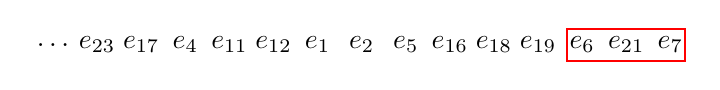
\begin{tikzpicture}[scale=0.8]
\tikzstyle{recti}=[rectangle,draw=red,thick,minimum width=1.5cm,minimum height=0.4cm]
\tikzstyle{stream}=[rectangle]
\node [stream] at (-0.7,0){$\dots$};
\node [stream] at (0,0) {$e_{23}$};
\node [stream] at (0.7,0) {$e_{17}$};
\node [stream] at (1.4,0) {$e_{4}$};
\node [stream] at (2.1,0) {$e_{11}$};
\node [stream] at (2.8,0) {$e_{12}$};
\node [stream] at (3.5,0) {$e_{1}$};
\node [stream] at (4.2,0) {$e_{2}$};
\node [stream] at (4.9,0) {$e_{5}$};
\node [stream] at (5.6,0) {$e_{16}$};
\node [stream] at (6.3,0) {$e_{18}$};
\node [stream] at (7.0,0) {$e_{19}$};
\node [stream] at (7.7,0) {$e_{6}$};
\node [stream] at (8.4,0) {$e_{21}$};
\node [stream] at (9.1,0) {$e_{7}$};
\node [recti] at (8.4,0) {};
\end{tikzpicture}
\end{center}

\end{frame}
\begin{frame}
\frametitle{The Adjacency Stream Model}
\framesubtitle{3}
\begin{center}
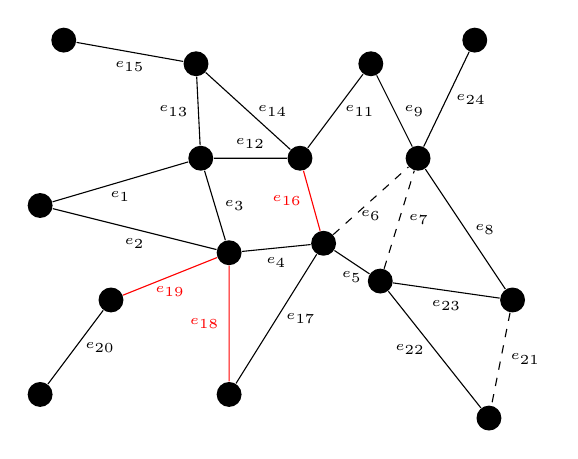
\begin{tikzpicture}[scale=0.6]
\tikzstyle{vertex}=[circle,fill=black,minimum size=9pt,inner sep=0pt]
\foreach \name/\point in {
	1/{-1,-1},
	2/{-1,3},
	3/{2.4,4},
	4/{5,2.2},
	5/{2.3,6},
	6/{6.2,1.4},
	7/{4.5,4},
	8/{-0.5,6.5},
	9/{3,-1},
	11/{3,2},
	10/{0.5,1},
	12/{6,6},
	13/{7,4},
	14/{9,1},
	15/{8.5,-1.5},
	16/{8.2,6.5}}
 	\node[vertex] (\name) at (\point) {};
\draw (2) -- (3) node[draw=none,fill=none,midway,below,font=\tiny] {$e_1$};
\draw (2) -- (11) node[draw=none,fill=none,midway,below,font=\tiny] {$e_2$};
\draw (3) -- (11) node[draw=none,fill=none,midway,right,font=\tiny] {$e_3$};
\draw (11) -- (4)node[draw=none,fill=none,midway,below,font=\tiny] {$e_4$};
\draw (4) -- (6)node[draw=none,fill=none,midway,below,font=\tiny] {$e_5$};
\draw[dashed] (4) -- (13)node[draw=none,fill=none,midway,below,font=\tiny] {$e_6$};
\draw[dashed] (6) -- (13)node[draw=none,fill=none,midway,right,font=\tiny] {$e_7$};
\draw (13) -- (14)node[draw=none,fill=none,midway,right,font=\tiny] {$e_8$};
\draw (13) -- (12)node[draw=none,fill=none,midway,right,font=\tiny] {$e_9$};
\draw (12) -- (7)node[draw=none,fill=none,midway,right,font=\tiny] {$e_{11}$};
\draw (7) -- (3)node[draw=none,fill=none,midway,above,font=\tiny] {$e_{12}$};
\draw (3) -- (5)node[draw=none,fill=none,midway,left,font=\tiny] {$e_{13}$};
\draw (5) -- (7)node[draw=none,fill=none,midway,right,font=\tiny] {$e_{14}$};
\draw (5) -- (8)node[draw=none,fill=none,midway,below,font=\tiny] {$e_{15}$};
\draw[red] (7) -- (4)node[draw=none,fill=none,midway,left,font=\tiny] {$e_{16}$};
\draw (9) -- (4)node[draw=none,fill=none,midway,right,font=\tiny] {$e_{17}$};
\draw[red] (11) -- (9)node[draw=none,fill=none,midway,left,font=\tiny] {$e_{18}$};
\draw[red] (11) -- (10)node[draw=none,fill=none,midway,below,font=\tiny] {$e_{19}$};
\draw (10) -- (1)node[draw=none,fill=none,midway,right,font=\tiny] {$e_{20}$};
\draw[dashed] (14) -- (15)node[draw=none,fill=none,midway,right,font=\tiny] {$e_{21}$};
\draw (6) -- (15)node[draw=none,fill=none,midway,left,font=\tiny] {$e_{22}$};
\draw (14) -- (6)node[draw=none,fill=none,midway,below,font=\tiny] {$e_{23}$};
\draw (13) -- (16)node[draw=none,fill=none,midway,right,font=\tiny] {$e_{24}$};
\end{tikzpicture}
\end{center}
\begin{center}
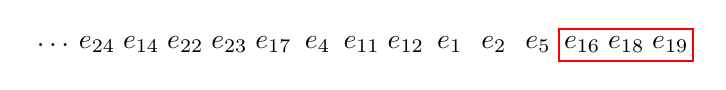
\begin{tikzpicture}[scale=0.8]
\tikzstyle{recti}=[rectangle,draw=red,thick,minimum width=1.7cm,minimum height=0.4cm]
\tikzstyle{stream}=[rectangle]
\node [stream] at (-0.7,0){$\dots$};
\node [stream] at (0,0) {$e_{24}$};
\node [stream] at (0.7,0) {$e_{14}$};
\node [stream] at (1.4,0) {$e_{22}$};
\node [stream] at (2.1,0) {$e_{23}$};
\node [stream] at (2.8,0) {$e_{17}$};
\node [stream] at (3.5,0) {$e_{4}$};
\node [stream] at (4.2,0) {$e_{11}$};
\node [stream] at (4.9,0) {$e_{12}$};
\node [stream] at (5.6,0) {$e_{1}$};
\node [stream] at (6.3,0) {$e_{2}$};
\node [stream] at (7.0,0) {$e_{5}$};
\node [stream] at (7.7,0) {$e_{16}$};
\node [stream] at (8.4,0) {$e_{18}$};
\node [stream] at (9.1,0) {$e_{19}$};
\node [recti] at (8.4,0) {};
\end{tikzpicture}
\end{center}
\end{frame}

\begin{frame}
\frametitle{Neighborhood Sampling}
\begin{itemize}
\item first sample a random edge $r_1$ from the edge stream
\item then sample a random edge $r_2$ from those edges that appear after $r_1$ and are adjacent to $r_1$
\item try to close $r_1$ and $r_2$ with a subsequent edge, to form a triangle $t$
\item simple data structure: $(r_1,r_2,t,c)$
\item sample $r_1$ and $r_2$ using \textit{reservoir sampling}
\end{itemize}

\end{frame}

\begin{frame}
\frametitle{The Algorithm}
\begin{algorithmic}
\State \textbf{Upon receiving edge} $e$ \textbf{at time step} $m$
\If {\text{\texttt{coin(1/$m$)}}="head"}
    \State $(r_1,r_2,t,c)=(e,\emptyset,\emptyset,0)$
\Else
	\If {$e$ is adjacent to $r_1$}
		\State $c\leftarrow c+1$
		\If {\texttt{coin(1/$c$)}="head"}
			\State $(r_2,t)\leftarrow(e,\emptyset)$
		\Else
			\If {$e$ forms a triangle with $r_1$ and $r_2$}
				\State $t\leftarrow \{r_1,r_2,e\}$
			\EndIf
		\EndIf
	\EndIf
\EndIf
\end{algorithmic}
\end{frame}

\begin{frame}
\frametitle{Example 1}
\begin{center}
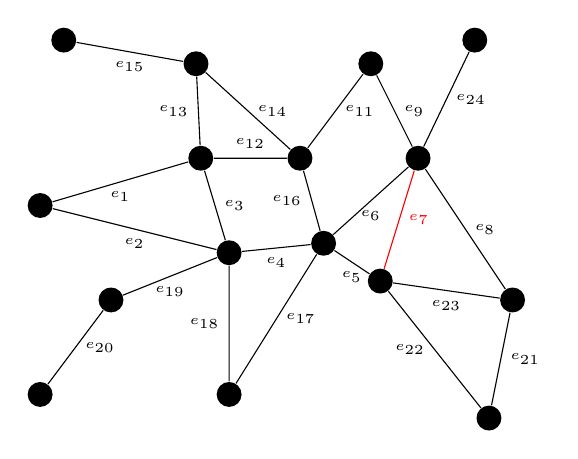
\begin{tikzpicture}[scale=0.6]
\tikzstyle{vertex}=[circle,fill=black,minimum size=9pt,inner sep=0pt]
\foreach \name/\point in {
	1/{-1,-1},
	2/{-1,3},
	3/{2.4,4},
	4/{5,2.2},
	5/{2.3,6},
	6/{6.2,1.4},
	7/{4.5,4},
	8/{-0.5,6.5},
	9/{3,-1},
	11/{3,2},
	10/{0.5,1},
	12/{6,6},
	13/{7,4},
	14/{9,1},
	15/{8.5,-1.5},
	16/{8.2,6.5}}
 	\node[vertex] (\name) at (\point) {};
\draw (2) -- (3) node[draw=none,fill=none,midway,below,font=\tiny] {$e_1$};
\draw (2) -- (11) node[draw=none,fill=none,midway,below,font=\tiny] {$e_2$};
\draw (3) -- (11) node[draw=none,fill=none,midway,right,font=\tiny] {$e_3$};
\draw (11) -- (4)node[draw=none,fill=none,midway,below,font=\tiny] {$e_4$};
\draw (4) -- (6)node[draw=none,fill=none,midway,below,font=\tiny] {$e_5$};
\draw (4) -- (13)node[draw=none,fill=none,midway,below,font=\tiny] {$e_6$};
\draw[red] (6) -- (13)node[draw=none,fill=none,midway,right,font=\tiny] {$e_7$};
\draw (13) -- (14)node[draw=none,fill=none,midway,right,font=\tiny] {$e_8$};
\draw (13) -- (12)node[draw=none,fill=none,midway,right,font=\tiny] {$e_9$};
\draw (12) -- (7)node[draw=none,fill=none,midway,right,font=\tiny] {$e_{11}$};
\draw (7) -- (3)node[draw=none,fill=none,midway,above,font=\tiny] {$e_{12}$};
\draw (3) -- (5)node[draw=none,fill=none,midway,left,font=\tiny] {$e_{13}$};
\draw (5) -- (7)node[draw=none,fill=none,midway,right,font=\tiny] {$e_{14}$};
\draw (5) -- (8)node[draw=none,fill=none,midway,below,font=\tiny] {$e_{15}$};
\draw (7) -- (4)node[draw=none,fill=none,midway,left,font=\tiny] {$e_{16}$};
\draw (9) -- (4)node[draw=none,fill=none,midway,right,font=\tiny] {$e_{17}$};
\draw (11) -- (9)node[draw=none,fill=none,midway,left,font=\tiny] {$e_{18}$};
\draw (11) -- (10)node[draw=none,fill=none,midway,below,font=\tiny] {$e_{19}$};
\draw (10) -- (1)node[draw=none,fill=none,midway,right,font=\tiny] {$e_{20}$};
\draw (14) -- (15)node[draw=none,fill=none,midway,right,font=\tiny] {$e_{21}$};
\draw (6) -- (15)node[draw=none,fill=none,midway,left,font=\tiny] {$e_{22}$};
\draw (14) -- (6)node[draw=none,fill=none,midway,below,font=\tiny] {$e_{23}$};
\draw (13) -- (16)node[draw=none,fill=none,midway,right,font=\tiny] {$e_{24}$};
\end{tikzpicture}
\end{center}
\begin{center}
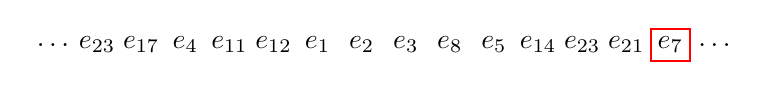
\begin{tikzpicture}[scale=0.8]
\tikzstyle{recti}=[rectangle,draw=red,thick,minimum width=0.5cm,minimum height=0.4cm]
\tikzstyle{stream}=[rectangle]
\node [stream] at (-0.7,0){$\dots$};
\node [stream] at (0,0) {$e_{23}$};
\node [stream] at (0.7,0) {$e_{17}$};
\node [stream] at (1.4,0) {$e_{4}$};
\node [stream] at (2.1,0) {$e_{11}$};
\node [stream] at (2.8,0) {$e_{12}$};
\node [stream] at (3.5,0) {$e_{1}$};
\node [stream] at (4.2,0) {$e_{2}$};
\node [stream] at (4.9,0) {$e_{3}$};
\node [stream] at (5.6,0) {$e_{8}$};
\node [stream] at (6.3,0) {$e_{5}$};
\node [stream] at (7.0,0) {$e_{14}$};
\node [stream] at (7.7,0) {$e_{23}$};
\node [stream] at (8.4,0) {$e_{21}$};
\node [stream] at (9.1,0) {$e_{7}$};
\node [stream] at (9.8,0) {$\dots$};
\node [recti] at (9.1,0) {};
\end{tikzpicture}
\end{center}
\vspace{-0.3cm}
$m=1042$\\
$estimator:$ $r_1=e_{15}$ $r_2=e_{39}$ $t=\emptyset$ $c=15$\\
\end{frame}


\begin{frame}
\frametitle{Example 2}
\begin{center}
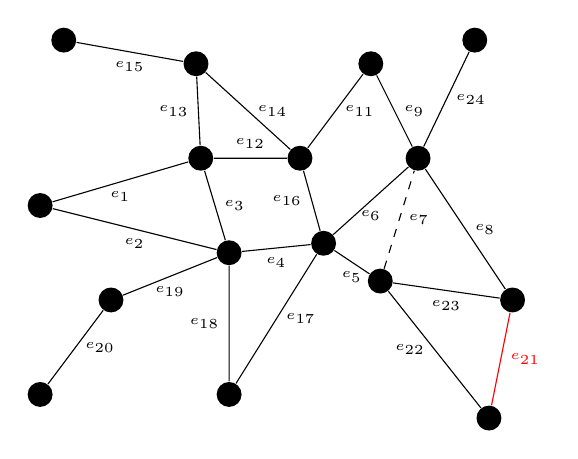
\begin{tikzpicture}[scale=0.6]
\tikzstyle{vertex}=[circle,fill=black,minimum size=9pt,inner sep=0pt]
\foreach \name/\point in {
	1/{-1,-1},
	2/{-1,3},
	3/{2.4,4},
	4/{5,2.2},
	5/{2.3,6},
	6/{6.2,1.4},
	7/{4.5,4},
	8/{-0.5,6.5},
	9/{3,-1},
	11/{3,2},
	10/{0.5,1},
	12/{6,6},
	13/{7,4},
	14/{9,1},
	15/{8.5,-1.5},
	16/{8.2,6.5}}
 	\node[vertex] (\name) at (\point) {};
\draw (2) -- (3) node[draw=none,fill=none,midway,below,font=\tiny] {$e_1$};
\draw (2) -- (11) node[draw=none,fill=none,midway,below,font=\tiny] {$e_2$};
\draw (3) -- (11) node[draw=none,fill=none,midway,right,font=\tiny] {$e_3$};
\draw (11) -- (4)node[draw=none,fill=none,midway,below,font=\tiny] {$e_4$};
\draw (4) -- (6)node[draw=none,fill=none,midway,below,font=\tiny] {$e_5$};
\draw (4) -- (13)node[draw=none,fill=none,midway,below,font=\tiny] {$e_6$};
\draw[dashed] (6) -- (13)node[draw=none,fill=none,midway,right,font=\tiny] {$e_7$};
\draw (13) -- (14)node[draw=none,fill=none,midway,right,font=\tiny] {$e_8$};
\draw (13) -- (12)node[draw=none,fill=none,midway,right,font=\tiny] {$e_9$};
\draw (12) -- (7)node[draw=none,fill=none,midway,right,font=\tiny] {$e_{11}$};
\draw (7) -- (3)node[draw=none,fill=none,midway,above,font=\tiny] {$e_{12}$};
\draw (3) -- (5)node[draw=none,fill=none,midway,left,font=\tiny] {$e_{13}$};
\draw (5) -- (7)node[draw=none,fill=none,midway,right,font=\tiny] {$e_{14}$};
\draw (5) -- (8)node[draw=none,fill=none,midway,below,font=\tiny] {$e_{15}$};
\draw (7) -- (4)node[draw=none,fill=none,midway,left,font=\tiny] {$e_{16}$};
\draw (9) -- (4)node[draw=none,fill=none,midway,right,font=\tiny] {$e_{17}$};
\draw (11) -- (9)node[draw=none,fill=none,midway,left,font=\tiny] {$e_{18}$};
\draw (11) -- (10)node[draw=none,fill=none,midway,below,font=\tiny] {$e_{19}$};
\draw (10) -- (1)node[draw=none,fill=none,midway,right,font=\tiny] {$e_{20}$};
\draw[red] (14) -- (15)node[draw=none,fill=none,midway,right,font=\tiny] {$e_{21}$};
\draw (6) -- (15)node[draw=none,fill=none,midway,left,font=\tiny] {$e_{22}$};
\draw (14) -- (6)node[draw=none,fill=none,midway,below,font=\tiny] {$e_{23}$};
\draw (13) -- (16)node[draw=none,fill=none,midway,right,font=\tiny] {$e_{24}$};
\end{tikzpicture}
\end{center}
\begin{center}
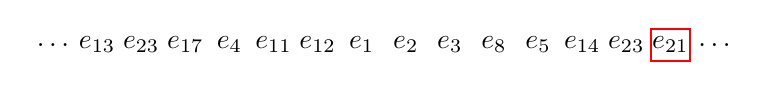
\begin{tikzpicture}[scale=0.8]
\tikzstyle{recti}=[rectangle,draw=red,thick,minimum width=0.5cm,minimum height=0.4cm]
\tikzstyle{stream}=[rectangle]
\node [stream] at (-0.7,0){$\dots$};
\node [stream] at (0,0) {$e_{13}$};
\node [stream] at (0.7,0) {$e_{23}$};
\node [stream] at (1.4,0) {$e_{17}$};
\node [stream] at (2.1,0) {$e_{4}$};
\node [stream] at (2.8,0) {$e_{11}$};
\node [stream] at (3.5,0) {$e_{12}$};
\node [stream] at (4.2,0) {$e_{1}$};
\node [stream] at (4.9,0) {$e_{2}$};
\node [stream] at (5.6,0) {$e_{3}$};
\node [stream] at (6.3,0) {$e_{8}$};
\node [stream] at (7.0,0) {$e_{5}$};
\node [stream] at (7.7,0) {$e_{14}$};
\node [stream] at (8.4,0) {$e_{23}$};
\node [stream] at (9.1,0) {$e_{21}$};
\node [stream] at (9.8,0) {$\dots$};
\node [recti] at (9.1,0) {};
\end{tikzpicture}
\end{center}
\vspace{-0.3cm}
$m=1043$\\
$estimator:$ $r_1=e_{7}$ $r_2=\emptyset$ $t=\emptyset$ $c=0$\\
\end{frame}

\begin{frame}
\frametitle{Example 3}
\begin{center}
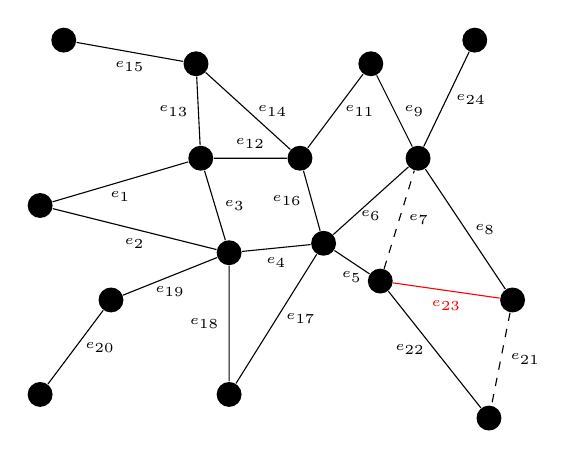
\begin{tikzpicture}[scale=0.6]
\tikzstyle{vertex}=[circle,fill=black,minimum size=9pt,inner sep=0pt]
\foreach \name/\point in {
	1/{-1,-1},
	2/{-1,3},
	3/{2.4,4},
	4/{5,2.2},
	5/{2.3,6},
	6/{6.2,1.4},
	7/{4.5,4},
	8/{-0.5,6.5},
	9/{3,-1},
	11/{3,2},
	10/{0.5,1},
	12/{6,6},
	13/{7,4},
	14/{9,1},
	15/{8.5,-1.5},
	16/{8.2,6.5}}
 	\node[vertex] (\name) at (\point) {};
\draw (2) -- (3) node[draw=none,fill=none,midway,below,font=\tiny] {$e_1$};
\draw (2) -- (11) node[draw=none,fill=none,midway,below,font=\tiny] {$e_2$};
\draw (3) -- (11) node[draw=none,fill=none,midway,right,font=\tiny] {$e_3$};
\draw (11) -- (4)node[draw=none,fill=none,midway,below,font=\tiny] {$e_4$};
\draw (4) -- (6)node[draw=none,fill=none,midway,below,font=\tiny] {$e_5$};
\draw (4) -- (13)node[draw=none,fill=none,midway,below,font=\tiny] {$e_6$};
\draw[dashed] (6) -- (13)node[draw=none,fill=none,midway,right,font=\tiny] {$e_7$};
\draw (13) -- (14)node[draw=none,fill=none,midway,right,font=\tiny] {$e_8$};
\draw (13) -- (12)node[draw=none,fill=none,midway,right,font=\tiny] {$e_9$};
\draw (12) -- (7)node[draw=none,fill=none,midway,right,font=\tiny] {$e_{11}$};
\draw (7) -- (3)node[draw=none,fill=none,midway,above,font=\tiny] {$e_{12}$};
\draw (3) -- (5)node[draw=none,fill=none,midway,left,font=\tiny] {$e_{13}$};
\draw (5) -- (7)node[draw=none,fill=none,midway,right,font=\tiny] {$e_{14}$};
\draw (5) -- (8)node[draw=none,fill=none,midway,below,font=\tiny] {$e_{15}$};
\draw (7) -- (4)node[draw=none,fill=none,midway,left,font=\tiny] {$e_{16}$};
\draw (9) -- (4)node[draw=none,fill=none,midway,right,font=\tiny] {$e_{17}$};
\draw (11) -- (9)node[draw=none,fill=none,midway,left,font=\tiny] {$e_{18}$};
\draw (11) -- (10)node[draw=none,fill=none,midway,below,font=\tiny] {$e_{19}$};
\draw (10) -- (1)node[draw=none,fill=none,midway,right,font=\tiny] {$e_{20}$};
\draw[dashed] (14) -- (15)node[draw=none,fill=none,midway,right,font=\tiny] {$e_{21}$};
\draw (6) -- (15)node[draw=none,fill=none,midway,left,font=\tiny] {$e_{22}$};
\draw[red] (14) -- (6)node[draw=none,fill=none,midway,below,font=\tiny] {$e_{23}$};
\draw (13) -- (16)node[draw=none,fill=none,midway,right,font=\tiny] {$e_{24}$};
\end{tikzpicture}
\end{center}
\begin{center}
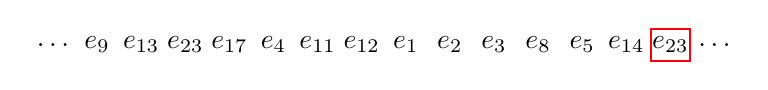
\begin{tikzpicture}[scale=0.8]
\tikzstyle{recti}=[rectangle,draw=red,thick,minimum width=0.5cm,minimum height=0.4cm]
\tikzstyle{stream}=[rectangle]
\node [stream] at (-0.7,0){$\dots$};
\node [stream] at (0,0) {$e_{9}$};
\node [stream] at (0.7,0) {$e_{13}$};
\node [stream] at (1.4,0) {$e_{23}$};
\node [stream] at (2.1,0) {$e_{17}$};
\node [stream] at (2.8,0) {$e_{4}$};
\node [stream] at (3.5,0) {$e_{11}$};
\node [stream] at (4.2,0) {$e_{12}$};
\node [stream] at (4.9,0) {$e_{1}$};
\node [stream] at (5.6,0) {$e_{2}$};
\node [stream] at (6.3,0) {$e_{3}$};
\node [stream] at (7.0,0) {$e_{8}$};
\node [stream] at (7.7,0) {$e_{5}$};
\node [stream] at (8.4,0) {$e_{14}$};
\node [stream] at (9.1,0) {$e_{23}$};
\node [stream] at (9.8,0) {$\dots$};
\node [recti] at (9.1,0) {};
\end{tikzpicture}
\end{center}
\vspace{-0.3cm}
$m=1044$\\
$estimator:$ $r_1=e_{7}$ $r_2=e_{23}$ $t=\emptyset$ $c=1$\\
\end{frame}

\begin{frame}
\frametitle{Example 4}
\begin{center}
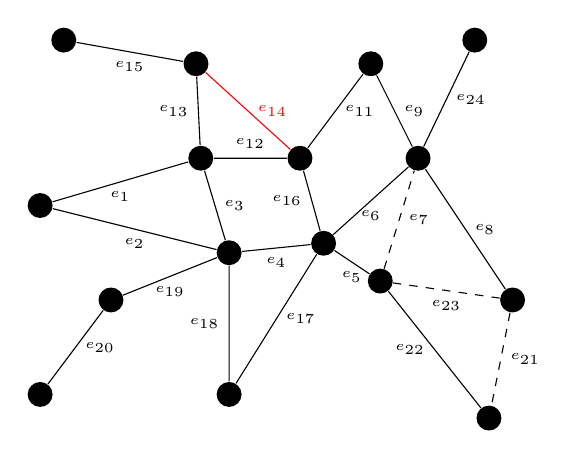
\begin{tikzpicture}[scale=0.6]
\tikzstyle{vertex}=[circle,fill=black,minimum size=9pt,inner sep=0pt]
\foreach \name/\point in {
	1/{-1,-1},
	2/{-1,3},
	3/{2.4,4},
	4/{5,2.2},
	5/{2.3,6},
	6/{6.2,1.4},
	7/{4.5,4},
	8/{-0.5,6.5},
	9/{3,-1},
	11/{3,2},
	10/{0.5,1},
	12/{6,6},
	13/{7,4},
	14/{9,1},
	15/{8.5,-1.5},
	16/{8.2,6.5}}
 	\node[vertex] (\name) at (\point) {};
\draw (2) -- (3) node[draw=none,fill=none,midway,below,font=\tiny] {$e_1$};
\draw (2) -- (11) node[draw=none,fill=none,midway,below,font=\tiny] {$e_2$};
\draw (3) -- (11) node[draw=none,fill=none,midway,right,font=\tiny] {$e_3$};
\draw (11) -- (4)node[draw=none,fill=none,midway,below,font=\tiny] {$e_4$};
\draw (4) -- (6)node[draw=none,fill=none,midway,below,font=\tiny] {$e_5$};
\draw (4) -- (13)node[draw=none,fill=none,midway,below,font=\tiny] {$e_6$};
\draw[dashed] (6) -- (13)node[draw=none,fill=none,midway,right,font=\tiny] {$e_7$};
\draw (13) -- (14)node[draw=none,fill=none,midway,right,font=\tiny] {$e_8$};
\draw (13) -- (12)node[draw=none,fill=none,midway,right,font=\tiny] {$e_9$};
\draw (12) -- (7)node[draw=none,fill=none,midway,right,font=\tiny] {$e_{11}$};
\draw (7) -- (3)node[draw=none,fill=none,midway,above,font=\tiny] {$e_{12}$};
\draw (3) -- (5)node[draw=none,fill=none,midway,left,font=\tiny] {$e_{13}$};
\draw[red] (5) -- (7)node[draw=none,fill=none,midway,right,font=\tiny] {$e_{14}$};
\draw (5) -- (8)node[draw=none,fill=none,midway,below,font=\tiny] {$e_{15}$};
\draw (7) -- (4)node[draw=none,fill=none,midway,left,font=\tiny] {$e_{16}$};
\draw (9) -- (4)node[draw=none,fill=none,midway,right,font=\tiny] {$e_{17}$};
\draw (11) -- (9)node[draw=none,fill=none,midway,left,font=\tiny] {$e_{18}$};
\draw (11) -- (10)node[draw=none,fill=none,midway,below,font=\tiny] {$e_{19}$};
\draw (10) -- (1)node[draw=none,fill=none,midway,right,font=\tiny] {$e_{20}$};
\draw[dashed] (14) -- (15)node[draw=none,fill=none,midway,right,font=\tiny] {$e_{21}$};
\draw (6) -- (15)node[draw=none,fill=none,midway,left,font=\tiny] {$e_{22}$};
\draw[dashed] (14) -- (6)node[draw=none,fill=none,midway,below,font=\tiny] {$e_{23}$};
\draw (13) -- (16)node[draw=none,fill=none,midway,right,font=\tiny] {$e_{24}$};
\end{tikzpicture}
\end{center}
\begin{center}
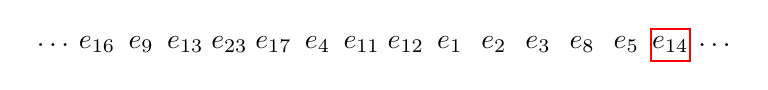
\begin{tikzpicture}[scale=0.8]
\tikzstyle{recti}=[rectangle,draw=red,thick,minimum width=0.5cm,minimum height=0.4cm]
\tikzstyle{stream}=[rectangle]
\node [stream] at (-0.7,0){$\dots$};
\node [stream] at (0,0) {$e_{16}$};
\node [stream] at (0.7,0) {$e_{9}$};
\node [stream] at (1.4,0) {$e_{13}$};
\node [stream] at (2.1,0) {$e_{23}$};
\node [stream] at (2.8,0) {$e_{17}$};
\node [stream] at (3.5,0) {$e_{4}$};
\node [stream] at (4.2,0) {$e_{11}$};
\node [stream] at (4.9,0) {$e_{12}$};
\node [stream] at (5.6,0) {$e_{1}$};
\node [stream] at (6.3,0) {$e_{2}$};
\node [stream] at (7.0,0) {$e_{3}$};
\node [stream] at (7.7,0) {$e_{8}$};
\node [stream] at (8.4,0) {$e_{5}$};
\node [stream] at (9.1,0) {$e_{14}$};
\node [stream] at (9.8,0) {$\dots$};
\node [recti] at (9.1,0) {};
\end{tikzpicture}
\end{center}
\vspace{-0.3cm}
$m=1045$\\
$estimator:$ $r_1=e_{7}$ $r_2=e_{23}$ $t=\emptyset$ $c=1$\\
\end{frame}

\begin{frame}
\frametitle{Example 5}
\begin{center}
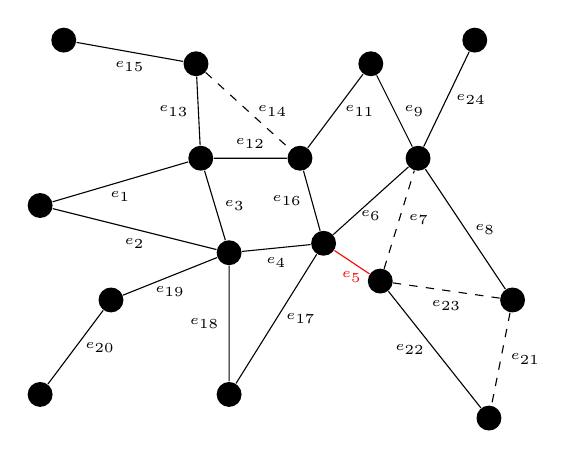
\begin{tikzpicture}[scale=0.6]
\tikzstyle{vertex}=[circle,fill=black,minimum size=9pt,inner sep=0pt]
\foreach \name/\point in {
	1/{-1,-1},
	2/{-1,3},
	3/{2.4,4},
	4/{5,2.2},
	5/{2.3,6},
	6/{6.2,1.4},
	7/{4.5,4},
	8/{-0.5,6.5},
	9/{3,-1},
	11/{3,2},
	10/{0.5,1},
	12/{6,6},
	13/{7,4},
	14/{9,1},
	15/{8.5,-1.5},
	16/{8.2,6.5}}
 	\node[vertex] (\name) at (\point) {};
\draw (2) -- (3) node[draw=none,fill=none,midway,below,font=\tiny] {$e_1$};
\draw (2) -- (11) node[draw=none,fill=none,midway,below,font=\tiny] {$e_2$};
\draw (3) -- (11) node[draw=none,fill=none,midway,right,font=\tiny] {$e_3$};
\draw (11) -- (4)node[draw=none,fill=none,midway,below,font=\tiny] {$e_4$};
\draw[red] (4) -- (6)node[draw=none,fill=none,midway,below,font=\tiny] {$e_5$};
\draw (4) -- (13)node[draw=none,fill=none,midway,below,font=\tiny] {$e_6$};
\draw[dashed] (6) -- (13)node[draw=none,fill=none,midway,right,font=\tiny] {$e_7$};
\draw (13) -- (14)node[draw=none,fill=none,midway,right,font=\tiny] {$e_8$};
\draw (13) -- (12)node[draw=none,fill=none,midway,right,font=\tiny] {$e_9$};
\draw (12) -- (7)node[draw=none,fill=none,midway,right,font=\tiny] {$e_{11}$};
\draw (7) -- (3)node[draw=none,fill=none,midway,above,font=\tiny] {$e_{12}$};
\draw (3) -- (5)node[draw=none,fill=none,midway,left,font=\tiny] {$e_{13}$};
\draw[dashed] (5) -- (7)node[draw=none,fill=none,midway,right,font=\tiny] {$e_{14}$};
\draw (5) -- (8)node[draw=none,fill=none,midway,below,font=\tiny] {$e_{15}$};
\draw (7) -- (4)node[draw=none,fill=none,midway,left,font=\tiny] {$e_{16}$};
\draw (9) -- (4)node[draw=none,fill=none,midway,right,font=\tiny] {$e_{17}$};
\draw (11) -- (9)node[draw=none,fill=none,midway,left,font=\tiny] {$e_{18}$};
\draw (11) -- (10)node[draw=none,fill=none,midway,below,font=\tiny] {$e_{19}$};
\draw (10) -- (1)node[draw=none,fill=none,midway,right,font=\tiny] {$e_{20}$};
\draw[dashed] (14) -- (15)node[draw=none,fill=none,midway,right,font=\tiny] {$e_{21}$};
\draw (6) -- (15)node[draw=none,fill=none,midway,left,font=\tiny] {$e_{22}$};
\draw[dashed] (14) -- (6)node[draw=none,fill=none,midway,below,font=\tiny] {$e_{23}$};
\draw (13) -- (16)node[draw=none,fill=none,midway,right,font=\tiny] {$e_{24}$};
\end{tikzpicture}
\end{center}
\begin{center}
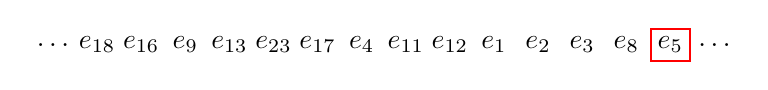
\begin{tikzpicture}[scale=0.8]
\tikzstyle{recti}=[rectangle,draw=red,thick,minimum width=0.5cm,minimum height=0.4cm]
\tikzstyle{stream}=[rectangle]
\node [stream] at (-0.7,0){$\dots$};
\node [stream] at (0,0) {$e_{18}$};
\node [stream] at (0.7,0) {$e_{16}$};
\node [stream] at (1.4,0) {$e_{9}$};
\node [stream] at (2.1,0) {$e_{13}$};
\node [stream] at (2.8,0) {$e_{23}$};
\node [stream] at (3.5,0) {$e_{17}$};
\node [stream] at (4.2,0) {$e_{4}$};
\node [stream] at (4.9,0) {$e_{11}$};
\node [stream] at (5.6,0) {$e_{12}$};
\node [stream] at (6.3,0) {$e_{1}$};
\node [stream] at (7.0,0) {$e_{2}$};
\node [stream] at (7.7,0) {$e_{3}$};
\node [stream] at (8.4,0) {$e_{8}$};
\node [stream] at (9.1,0) {$e_{5}$};
\node [stream] at (9.8,0) {$\dots$};
\node [recti] at (9.1,0) {};
\end{tikzpicture}
\end{center}
\vspace{-0.3cm}
$m=1046$\\
$estimator:$ $r_1=e_{7}$ $r_2=e_{23}$ $t=\emptyset$ $c=2$\\
\end{frame}

\begin{frame}
\frametitle{Example 6}
\begin{center}
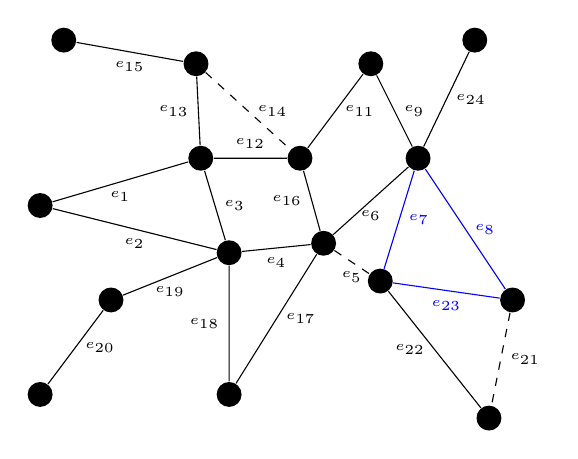
\begin{tikzpicture}[scale=0.6]
\tikzstyle{vertex}=[circle,fill=black,minimum size=9pt,inner sep=0pt]
\foreach \name/\point in {
	1/{-1,-1},
	2/{-1,3},
	3/{2.4,4},
	4/{5,2.2},
	5/{2.3,6},
	6/{6.2,1.4},
	7/{4.5,4},
	8/{-0.5,6.5},
	9/{3,-1},
	11/{3,2},
	10/{0.5,1},
	12/{6,6},
	13/{7,4},
	14/{9,1},
	15/{8.5,-1.5},
	16/{8.2,6.5}}
 	\node[vertex] (\name) at (\point) {};
\draw (2) -- (3) node[draw=none,fill=none,midway,below,font=\tiny] {$e_1$};
\draw (2) -- (11) node[draw=none,fill=none,midway,below,font=\tiny] {$e_2$};
\draw (3) -- (11) node[draw=none,fill=none,midway,right,font=\tiny] {$e_3$};
\draw (11) -- (4)node[draw=none,fill=none,midway,below,font=\tiny] {$e_4$};
\draw[dashed] (4) -- (6)node[draw=none,fill=none,midway,below,font=\tiny] {$e_5$};
\draw (4) -- (13)node[draw=none,fill=none,midway,below,font=\tiny] {$e_6$};
\draw[blue] (6) -- (13)node[draw=none,fill=none,midway,right,font=\tiny] {$e_7$};
\draw[blue] (13) -- (14)node[draw=none,fill=none,midway,right,font=\tiny] {$e_8$};
\draw (13) -- (12)node[draw=none,fill=none,midway,right,font=\tiny] {$e_9$};
\draw (12) -- (7)node[draw=none,fill=none,midway,right,font=\tiny] {$e_{11}$};
\draw (7) -- (3)node[draw=none,fill=none,midway,above,font=\tiny] {$e_{12}$};
\draw (3) -- (5)node[draw=none,fill=none,midway,left,font=\tiny] {$e_{13}$};
\draw[dashed] (5) -- (7)node[draw=none,fill=none,midway,right,font=\tiny] {$e_{14}$};
\draw (5) -- (8)node[draw=none,fill=none,midway,below,font=\tiny] {$e_{15}$};
\draw (7) -- (4)node[draw=none,fill=none,midway,left,font=\tiny] {$e_{16}$};
\draw (9) -- (4)node[draw=none,fill=none,midway,right,font=\tiny] {$e_{17}$};
\draw (11) -- (9)node[draw=none,fill=none,midway,left,font=\tiny] {$e_{18}$};
\draw (11) -- (10)node[draw=none,fill=none,midway,below,font=\tiny] {$e_{19}$};
\draw (10) -- (1)node[draw=none,fill=none,midway,right,font=\tiny] {$e_{20}$};
\draw[dashed] (14) -- (15)node[draw=none,fill=none,midway,right,font=\tiny] {$e_{21}$};
\draw (6) -- (15)node[draw=none,fill=none,midway,left,font=\tiny] {$e_{22}$};
\draw[blue] (14) -- (6)node[draw=none,fill=none,midway,below,font=\tiny] {$e_{23}$};
\draw (13) -- (16)node[draw=none,fill=none,midway,right,font=\tiny] {$e_{24}$};
\end{tikzpicture}
\end{center}
\begin{center}
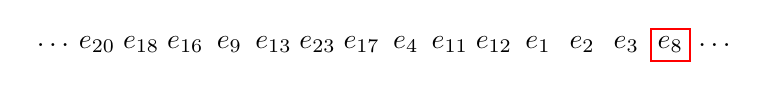
\begin{tikzpicture}[scale=0.8]
\tikzstyle{recti}=[rectangle,draw=red,thick,minimum width=0.5cm,minimum height=0.4cm]
\tikzstyle{stream}=[rectangle]
\node [stream] at (-0.7,0){$\dots$};
\node [stream] at (0,0) {$e_{20}$};
\node [stream] at (0.7,0) {$e_{18}$};
\node [stream] at (1.4,0) {$e_{16}$};
\node [stream] at (2.1,0) {$e_{9}$};
\node [stream] at (2.8,0) {$e_{13}$};
\node [stream] at (3.5,0) {$e_{23}$};
\node [stream] at (4.2,0) {$e_{17}$};
\node [stream] at (4.9,0) {$e_{4}$};
\node [stream] at (5.6,0) {$e_{11}$};
\node [stream] at (6.3,0) {$e_{12}$};
\node [stream] at (7.0,0) {$e_{1}$};
\node [stream] at (7.7,0) {$e_{2}$};
\node [stream] at (8.4,0) {$e_{3}$};
\node [stream] at (9.1,0) {$e_{8}$};
\node [stream] at (9.8,0) {$\dots$};
\node [recti] at (9.1,0) {};
\end{tikzpicture}
\end{center}
\vspace{-0.3cm}
$m=1047$\\
$estimator:$ $r_1=e_{7}$ $r_2=e_{23}$ $t=\{e_7,e_{23},e_8\}$ $c=3$\\
\end{frame}

\section{Counting Triangles}
\begin{frame}
\frametitle{Expectation value of $\tau$}
\begin{itemize}
\item We want to find the number of triangles $\tau(G)$
\item Let $t$ and $c$ be the values the neighborhood sampling algorithm maintains and $m$ be the number of edges observed so far. Define:
\begin{center}
$\tilde{\tau}=\begin{cases}c\times m & \text{if }t\neq \emptyset\\0 & \text{otherwise}\end{cases}$\\
\end{center}
Then $\text{\textbf{E}}[\tilde{\tau}]=\tau(G)$
\end{itemize}
\end{frame}

\begin{frame}
\frametitle{An $(\epsilon,\delta)$-approximation to the triangle count}
\begin{itemize}
\item Take the average of $r$ such estimators with
\item With probability $1-\delta$ the average of the estimators is in 
\begin{center}
$[(1-\epsilon)\tau(G),(1+\epsilon)\tau(G)]$
\end{center}
\pause
\item  Relation between number of estimators and error of the approximation:
\begin{center}
$r\geq\frac{6}{\epsilon^2}\frac{m\Delta}{\tau(G)}log(\frac{2}{\delta})$
\end{center}
\item LiveJournal:
\begin{itemize}
\item given \mbox{$m=34.7M, \Delta=14815, \tau(G)=177,820,130$}
\item chose $\epsilon=0.1, \delta=0.05$
\item then $r\geq6.3M$
\end{itemize}
\end{itemize}
\end{frame}
\begin{frame}
\begin{minipage}[t]{0.48\linewidth}
\begin{center}
%\vspace{-2cm}
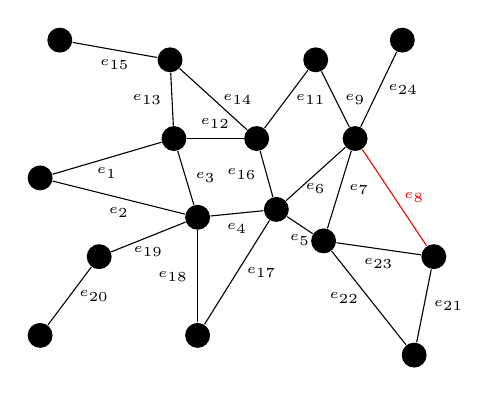
\begin{tikzpicture}[scale=0.5]
\tikzstyle{vertex}=[circle,fill=black,minimum size=9pt,inner sep=0pt]
\foreach \name/\point in {
	1/{-1,-1},
	2/{-1,3},
	3/{2.4,4},
	4/{5,2.2},
	5/{2.3,6},
	6/{6.2,1.4},
	7/{4.5,4},
	8/{-0.5,6.5},
	9/{3,-1},
	11/{3,2},
	10/{0.5,1},
	12/{6,6},
	13/{7,4},
	14/{9,1},
	15/{8.5,-1.5},
	16/{8.2,6.5}}
 	\node[vertex] (\name) at (\point) {};
\draw (2) -- (3) node[draw=none,fill=none,midway,below,font=\tiny] {$e_1$};
\draw (2) -- (11) node[draw=none,fill=none,midway,below,font=\tiny] {$e_2$};
\draw (3) -- (11) node[draw=none,fill=none,midway,right,font=\tiny] {$e_3$};
\draw (11) -- (4)node[draw=none,fill=none,midway,below,font=\tiny] {$e_4$};
\draw (4) -- (6)node[draw=none,fill=none,midway,below,font=\tiny] {$e_5$};
\draw (4) -- (13)node[draw=none,fill=none,midway,below,font=\tiny] {$e_6$};
\draw (6) -- (13)node[draw=none,fill=none,midway,right,font=\tiny] {$e_7$};
\draw[red] (13) -- (14)node[draw=none,fill=none,midway,right,font=\tiny] {$e_8$};
\draw (13) -- (12)node[draw=none,fill=none,midway,right,font=\tiny] {$e_9$};
\draw (12) -- (7)node[draw=none,fill=none,midway,right,font=\tiny] {$e_{11}$};
\draw (7) -- (3)node[draw=none,fill=none,midway,above,font=\tiny] {$e_{12}$};
\draw (3) -- (5)node[draw=none,fill=none,midway,left,font=\tiny] {$e_{13}$};
\draw (5) -- (7)node[draw=none,fill=none,midway,right,font=\tiny] {$e_{14}$};
\draw (5) -- (8)node[draw=none,fill=none,midway,below,font=\tiny] {$e_{15}$};
\draw (7) -- (4)node[draw=none,fill=none,midway,left,font=\tiny] {$e_{16}$};
\draw (9) -- (4)node[draw=none,fill=none,midway,right,font=\tiny] {$e_{17}$};
\draw (11) -- (9)node[draw=none,fill=none,midway,left,font=\tiny] {$e_{18}$};
\draw (11) -- (10)node[draw=none,fill=none,midway,below,font=\tiny] {$e_{19}$};
\draw (10) -- (1)node[draw=none,fill=none,midway,right,font=\tiny] {$e_{20}$};
\draw (14) -- (15)node[draw=none,fill=none,midway,right,font=\tiny] {$e_{21}$};
\draw (6) -- (15)node[draw=none,fill=none,midway,left,font=\tiny] {$e_{22}$};
\draw (14) -- (6)node[draw=none,fill=none,midway,below,font=\tiny] {$e_{23}$};
\draw (13) -- (16)node[draw=none,fill=none,midway,right,font=\tiny] {$e_{24}$};
\end{tikzpicture}
\end{center}
$m=1042$
\begin{center}
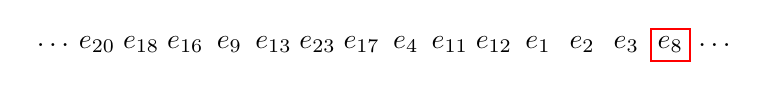
\begin{tikzpicture}[scale=0.8]
\tikzstyle{recti}=[rectangle,draw=red,thick,minimum width=0.5cm,minimum height=0.4cm]
\tikzstyle{stream}=[rectangle]
\node [stream] at (-0.7,0){$\dots$};
\node [stream] at (0,0) {$e_{20}$};
\node [stream] at (0.7,0) {$e_{18}$};
\node [stream] at (1.4,0) {$e_{16}$};
\node [stream] at (2.1,0) {$e_{9}$};
\node [stream] at (2.8,0) {$e_{13}$};
\node [stream] at (3.5,0) {$e_{23}$};
\node [stream] at (4.2,0) {$e_{17}$};
\node [stream] at (4.9,0) {$e_{4}$};
\node [stream] at (5.6,0) {$e_{11}$};
\node [stream] at (6.3,0) {$e_{12}$};
\node [stream] at (7.0,0) {$e_{1}$};
\node [stream] at (7.7,0) {$e_{2}$};
\node [stream] at (8.4,0) {$e_{3}$};
\node [stream] at (9.1,0) {$e_{8}$};
\node [stream] at (9.8,0) {$\dots$};
\node [recti] at (9.1,0) {};
\end{tikzpicture}
\end{center}
\end{minipage}\hfill
\begin{minipage}[t]{0.48\linewidth}
\tiny$estimator1:$ $r_1=e_{101}$ $r_2=\emptyset$ $t=\emptyset$ $c=0$\\
$estimator2:$ $r_1=e_{9}$ $r_2=e_{23}$ $t=\emptyset$ $c=13$\\
$estimator3:$ $r_1=e_{8}$ $r_2=\emptyset$ $t=\emptyset$ $c=33$\\
\mbox{$estimator4:$ $r_1=e_{99}$ $r_2=e_{42}$ $t=\{e_{99},e_{42},e_{101}\}$ $c=33$}\\
$estimator5:$ $r_1=e_{7}$ $r_2=\emptyset$ $t=\emptyset$ $c=0$\\
\mbox{$estimator6:$ $r_1=e_{8}$ $r_2=e_{23}$ $t=\{e_7,e_{23},e_8\}$ $c=31$}\\
$estimator7:$ $r_1=e_{42}$ $r_2=\emptyset$ $t=\emptyset$ $c=0$\\
\mbox{$estimator8:$ $r_1=e_{17}$ $r_2=e_{42}$ $t=\{e_{17},e_{42},e_{23}\}$ $c=92$}\\
\begin{center}
$\vdots$\\
$\vdots$
\end{center}
\end{minipage}

\end{frame}

\begin{frame}
\begin{minipage}[t]{0.48\linewidth}
\begin{center}
%\vspace{-2cm}
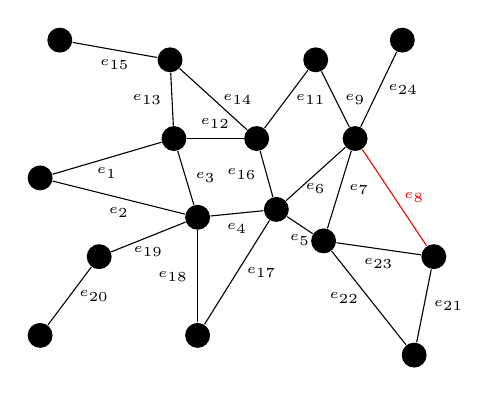
\begin{tikzpicture}[scale=0.5]
\tikzstyle{vertex}=[circle,fill=black,minimum size=9pt,inner sep=0pt]
\foreach \name/\point in {
	1/{-1,-1},
	2/{-1,3},
	3/{2.4,4},
	4/{5,2.2},
	5/{2.3,6},
	6/{6.2,1.4},
	7/{4.5,4},
	8/{-0.5,6.5},
	9/{3,-1},
	11/{3,2},
	10/{0.5,1},
	12/{6,6},
	13/{7,4},
	14/{9,1},
	15/{8.5,-1.5},
	16/{8.2,6.5}}
 	\node[vertex] (\name) at (\point) {};
\draw (2) -- (3) node[draw=none,fill=none,midway,below,font=\tiny] {$e_1$};
\draw (2) -- (11) node[draw=none,fill=none,midway,below,font=\tiny] {$e_2$};
\draw (3) -- (11) node[draw=none,fill=none,midway,right,font=\tiny] {$e_3$};
\draw (11) -- (4)node[draw=none,fill=none,midway,below,font=\tiny] {$e_4$};
\draw (4) -- (6)node[draw=none,fill=none,midway,below,font=\tiny] {$e_5$};
\draw (4) -- (13)node[draw=none,fill=none,midway,below,font=\tiny] {$e_6$};
\draw (6) -- (13)node[draw=none,fill=none,midway,right,font=\tiny] {$e_7$};
\draw[red] (13) -- (14)node[draw=none,fill=none,midway,right,font=\tiny] {$e_8$};
\draw (13) -- (12)node[draw=none,fill=none,midway,right,font=\tiny] {$e_9$};
\draw (12) -- (7)node[draw=none,fill=none,midway,right,font=\tiny] {$e_{11}$};
\draw (7) -- (3)node[draw=none,fill=none,midway,above,font=\tiny] {$e_{12}$};
\draw (3) -- (5)node[draw=none,fill=none,midway,left,font=\tiny] {$e_{13}$};
\draw (5) -- (7)node[draw=none,fill=none,midway,right,font=\tiny] {$e_{14}$};
\draw (5) -- (8)node[draw=none,fill=none,midway,below,font=\tiny] {$e_{15}$};
\draw (7) -- (4)node[draw=none,fill=none,midway,left,font=\tiny] {$e_{16}$};
\draw (9) -- (4)node[draw=none,fill=none,midway,right,font=\tiny] {$e_{17}$};
\draw (11) -- (9)node[draw=none,fill=none,midway,left,font=\tiny] {$e_{18}$};
\draw (11) -- (10)node[draw=none,fill=none,midway,below,font=\tiny] {$e_{19}$};
\draw (10) -- (1)node[draw=none,fill=none,midway,right,font=\tiny] {$e_{20}$};
\draw (14) -- (15)node[draw=none,fill=none,midway,right,font=\tiny] {$e_{21}$};
\draw (6) -- (15)node[draw=none,fill=none,midway,left,font=\tiny] {$e_{22}$};
\draw (14) -- (6)node[draw=none,fill=none,midway,below,font=\tiny] {$e_{23}$};
\draw (13) -- (16)node[draw=none,fill=none,midway,right,font=\tiny] {$e_{24}$};
\end{tikzpicture}
\end{center}
$m=1042$

\end{minipage}\hfill
\begin{minipage}[t]{0.48\linewidth}
\tiny$estimator1:$ $r_1=e_{101}$ $r_2=\emptyset$ $t=\emptyset$ $c=0$\\
$estimator2:$ $r_1=e_{9}$ $r_2=e_{23}$ $t=\emptyset$ $c=13$\\
$estimator3:$ $r_1=e_{8}$ $r_2=\emptyset$ $t=\emptyset$ $c=33$\\
\mbox{$estimator4:$ $r_1=e_{99}$ $r_2=e_{42}$ $t=\{e_{99},e_{42},e_{101}\}$ $c=33$}\\
$estimator5:$ $r_1=e_{7}$ $r_2=\emptyset$ $t=\emptyset$ $c=0$\\
\mbox{$estimator6:$ $r_1=e_{8}$ $r_2=e_{23}$ $t=\{e_7,e_{23},e_8\}$ $c=31$}\\
$estimator7:$ $r_1=e_{42}$ $r_2=\emptyset$ $t=\emptyset$ $c=0$\\
\mbox{$estimator8:$ $r_1=e_{17}$ $r_2=e_{42}$ $t=\{e_{17},e_{42},e_{23}\}$ $c=92$}\\
\begin{center}
$\vdots$\\
$\vdots$
\end{center}
\small
\vspace{1cm}
\end{minipage}
\begin{center}

$\tilde{\tau}=\begin{cases}c\times m & \text{if }t\neq \emptyset\\0 & \text{otherwise}\end{cases}$\\

\end{center}
\end{frame}
\section{Bulk Processing}
\begin{frame}
\frametitle{Nearly-Linear Time Triangle Counting}
\begin{itemize}
\item so far we have a $O(mr)$-time implemenation
\item with a small constant factor increase in space, we are able to achieve $O(m+r)$-time bound
\item \textbf{Bulk Processing} Process edges in bulk. Read $w$ edges at a time and update all estimators simultaneously.
\end{itemize}
\begin{center}
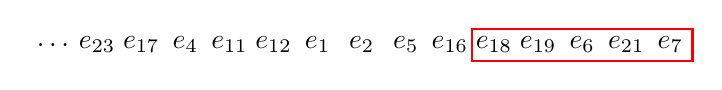
\begin{tikzpicture}[scale=0.8]
\tikzstyle{recti}=[rectangle,draw=red,thick,minimum width=2.8cm,minimum height=0.4cm]
\tikzstyle{stream}=[rectangle]
\node [stream] at (-0.7,0){$\dots$};
\node [stream] at (0,0) {$e_{23}$};
\node [stream] at (0.7,0) {$e_{17}$};
\node [stream] at (1.4,0) {$e_{4}$};
\node [stream] at (2.1,0) {$e_{11}$};
\node [stream] at (2.8,0) {$e_{12}$};
\node [stream] at (3.5,0) {$e_{1}$};
\node [stream] at (4.2,0) {$e_{2}$};
\node [stream] at (4.9,0) {$e_{5}$};
\node [stream] at (5.6,0) {$e_{16}$};
\node [stream] at (6.3,0) {$e_{18}$};
\node [stream] at (7.0,0) {$e_{19}$};
\node [stream] at (7.7,0) {$e_{6}$};
\node [stream] at (8.4,0) {$e_{21}$};
\node [stream] at (9.1,0) {$e_{7}$};
\node [recti] at (7.7,0) {};
\end{tikzpicture}
\end{center}
\end{frame}

\begin{frame}
\frametitle{Bulk Processing Step 1: Resample Level 1 edges}
\begin{itemize}
\item sample new $r_1$ edges from the batch of size $w$. Keep current edge with probability $\frac{m}{w+m}$ and with remaining probability, replace it with edge uniformly chosen from $B$.
\item for each estimator: draw random number between $1$ and $m+w$.
\begin{center}
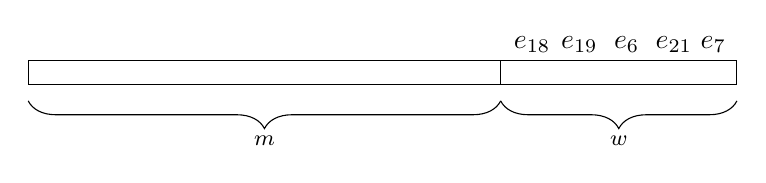
\begin{tikzpicture}
\tikzstyle{recti}=[rectangle,draw=red,thick,minimum width=2.8cm,minimum height=0.4cm]
\tikzstyle{stream}=[rectangle]
\draw[] (0,0) rectangle (6,0.3) node[pos=0.5]{};
\draw[] (6,0) rectangle (9,0.3) node[pos=0.5]{};
\node [stream] at (6.4,0.5) {$e_{18}$};
\node [stream] at (7.0,0.5) {$e_{19}$};
\node [stream] at (7.6,0.5) {$e_{6}$};
\node [stream] at (8.2,0.5) {$e_{21}$};
\node [stream] at (8.7,0.5) {$e_{7}$};
\draw [decorate,decoration={brace,amplitude=10pt,mirror},yshift=-6pt ]
(0,0) -- (6,0) node [black,midway,anchor=north,yshift=-9pt] {\footnotesize $m$};
\draw [decorate,decoration={brace,amplitude=10pt,mirror},yshift=-6pt ]
(6,0) -- (9,0) node [black,midway,anchor=north,yshift=-9pt] {\footnotesize $w$};
\end{tikzpicture}
\end{center}
\end{itemize}
\end{frame}

\begin{frame}
\frametitle{Bulk Processing Step 2: Identify Level-2 candidates and sample from them}
\begin{itemize}
\item The sample space we want to sample $r_2$ edges from, is those edges that are adjacent to $r_1$ and arrive after $r_1$.
\item Let $N(r_1)$ be those edges that arrive after $r_1$ in the stream.
\item Suppose for each estimator we have the following values ($r_1=(x,y)$):
\begin{itemize}
\item $\vert N(r_1)\vert=c^-+c^+$
\item $c^-$: $\#$ edges in $N(r_1)$ before the badge.
\item $c^+=a+b$:  $\#$ of edges in $N(r_1)$ inside the badge.
\item $a$: $\#$ of edges in $N(r_1)$, sharing endpoint $x$ with $r_1$, inside badge.
\item $b$: $\#$ of edges in $N(r_1)$, sharing endpoint $y$ with $r_1$, inside badge.
\end{itemize}
\end{itemize}
\end{frame}

\begin{frame}
\frametitle{Example: $c^-, c^+, a, b$}
\begin{minipage}[t]{0.48\linewidth}
\begin{center}
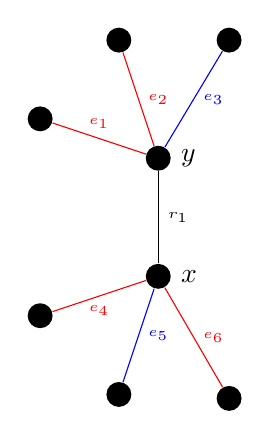
\begin{tikzpicture}[scale=0.5]
\tikzstyle{vertex}=[circle,fill=black,minimum size=9pt,inner sep=0pt]
\node[vertex,label=right:$y$] (1) at (4,3){};
\node[vertex,label=right:$x$] (2) at (4,0){};
\node[vertex] (3) at (1,4){};
\node[vertex] (4) at (3,6){};
\node[vertex] (5) at (1,-1){};
\node[vertex] (6) at (3,-3){};
\node[vertex] (7) at (5.8,6){};
\node[vertex] (8) at (5.8,-3.1){};
\draw (1) -- (2)node[draw=none,fill=none,midway,right,font=\tiny] {$r_1$};
\draw[red] (1) -- (3)node[draw=none,fill=none,midway,above,font=\tiny] {$e_1$};
\draw[red] (1) -- (4)node[draw=none,fill=none,midway,right,font=\tiny] {$e_2$};
\draw[blue] (1) -- (7)node[draw=none,fill=none,midway,right,font=\tiny] {$e_3$};
\draw[red] (2) -- (5)node[draw=none,fill=none,midway,below,font=\tiny] {$e_4$};
\draw[blue] (2) -- (6)node[draw=none,fill=none,midway,right,font=\tiny] {$e_5$};
\draw[red] (2) -- (8)node[draw=none,fill=none,midway,right,font=\tiny] {$e_6$};
\end{tikzpicture}
\end{center}

\begin{center}
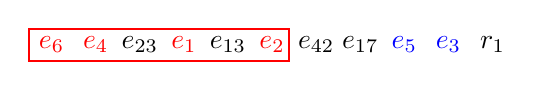
\begin{tikzpicture}[scale=0.8]
\tikzstyle{recti}=[rectangle,draw=red,thick,minimum width=3.3cm,minimum height=0.4cm]
\tikzstyle{stream}=[rectangle,]
\node [stream] at (6,0) {$r_1$};
\node [stream] at (5.3,0) {\color{blue}{$e_3$}};
\node [stream] at (4.6,0) {\color{blue}{$e_5$}};
\node [stream] at (3.9,0) {$e_{17}$};
\node [stream] at (3.2,0) {$e_{42}$};
\node [stream] at (2.5,0) {\color{red}{$e_2$}};
\node [stream] at (1.8,0) {$e_{13}$};
\node [stream] at (1.1,0) {\color{red}{$e_1$}};
\node [stream] at (0.4,0) {$e_{23}$};
\node [stream] at (-0.3,0) {\color{red}{$e_4$}};
\node [stream] at (-1.0,0) {\color{red}{$e_6$}};
\node [recti] at (0.7,0) {};
\end{tikzpicture}
\end{center}
\end{minipage}
\begin{minipage}[t]{0.48\linewidth}
\vspace{-4cm}
\begin{itemize}
\item $\vert N(r_1)\vert=c^-+c^+=6$
\item $c^-=2$
\item $c^+=a+b=4$
\item $a=2$
\item $b=2$
\pause
\item with probability $\frac{c^+}{c^++c^-}$ sample a $r_1$ adjacent edge from the badge as new $r_2$
\end{itemize}
\end{minipage}
\end{frame}

\begin{frame}
\frametitle{Sampling new $r_2$ edges from the badge}
\begin{itemize}
\item For each estimator draw random number $\varphi$ between 1 and $c^-+c^+$\\
\vspace{1cm}
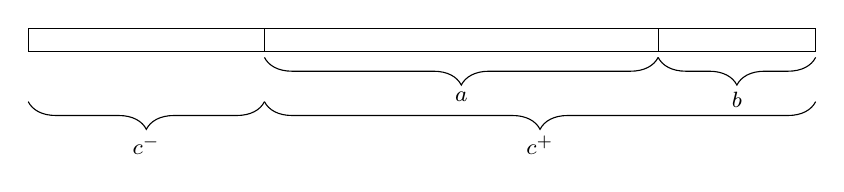
\begin{tikzpicture}
\draw[] (0,0) rectangle (3,0.3) node[pos=0.5]{};
\draw[] (3,0) rectangle (8,0.3) node[pos=0.5]{};
\draw[] (8,0) rectangle (10,0.3) node[pos=0.5]{};
\draw [decorate,decoration={brace,amplitude=10pt,mirror},yshift=-18pt ]
(0,0) -- (3,0) node [black,midway,anchor=north,yshift=-9pt] {\footnotesize $c^-$};
\draw [decorate,decoration={brace,amplitude=10pt,mirror},yshift=-2pt ]
(3,0) -- (8,0) node [black,midway,anchor=north,yshift=-9pt] {\footnotesize $a$};
\draw [decorate,decoration={brace,amplitude=10pt,mirror},yshift=-2pt ]
(8,0) -- (10,0) node [black,midway,anchor=north,yshift=-9pt] {\footnotesize $b$};
\draw [decorate,decoration={brace,amplitude=10pt,mirror},yshift=-18pt ]
(3,0) -- (10,0) node [black,midway,anchor=north,yshift=-9pt] {\footnotesize $c^+$};
\end{tikzpicture}
\item if $\varphi\leq c^-$ don't sample new $r_2$ edge
\item if $c^- \leq \varphi \leq c^-+a$ sample one of the edges that share endpoint $x$
\item else sample one of the edges that share endpoint $y$
\end{itemize}
\end{frame}

\begin{frame}
\frametitle{Sampling $r_2$ edges summary}
\begin{itemize}
\item paper presents simple algorithm to get $c^-, c^+, a, b$ which goes over the badge once
%\begin{itemize}
%\item keep hashtable that maps edges to estimators that hold it as $r_1$
%\item keep track how many edges were incident to $x$ and $y$ at time when $r_1$ arrived
%\item count how many edges are incident to $x$ and $y$ after all edges of badge arrived
%\item difference between two above values give $a$ and $b$
%\end{itemize}
\item then we go over all estimators to sample the $r_2$ edges
\item then go over badge again to find edge that corresponds to offset in range $c^-, c^-+a$ or $c^-+a,c^-+a+b$
\end{itemize}
\vspace{1cm}
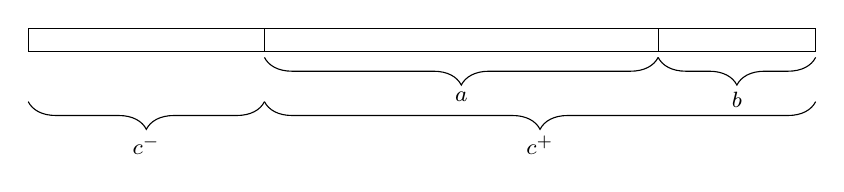
\begin{tikzpicture}
\draw[] (0,0) rectangle (3,0.3) node[pos=0.5]{};
\draw[] (3,0) rectangle (8,0.3) node[pos=0.5]{};
\draw[] (8,0) rectangle (10,0.3) node[pos=0.5]{};
\draw [decorate,decoration={brace,amplitude=10pt,mirror},yshift=-18pt ]
(0,0) -- (3,0) node [black,midway,anchor=north,yshift=-9pt] {\footnotesize $c^-$};
\draw [decorate,decoration={brace,amplitude=10pt,mirror},yshift=-2pt ]
(3,0) -- (8,0) node [black,midway,anchor=north,yshift=-9pt] {\footnotesize $a$};
\draw [decorate,decoration={brace,amplitude=10pt,mirror},yshift=-2pt ]
(8,0) -- (10,0) node [black,midway,anchor=north,yshift=-9pt] {\footnotesize $b$};
\draw [decorate,decoration={brace,amplitude=10pt,mirror},yshift=-18pt ]
(3,0) -- (10,0) node [black,midway,anchor=north,yshift=-9pt] {\footnotesize $c^+$};
\end{tikzpicture}
\end{frame}

\begin{frame}
\frametitle{Bulk Processing Step 3: Detect edges that close the wedges}
\begin{itemize}
\item For each estimator with $r_1$ and $r_2$ edges, check if badge contains an edge that comes after $r_2$ and closes $r_1, r_2$ to form a triangle
\item Create hashtable that maps the needed edges to the estimators.
\item Check if badge contains this edge and whether it comes after $r_2$	
\end{itemize}

\begin{minipage}[t]{0.31\linewidth}

\begin{center}
\mbox{\tiny {est.1: $r_1=e_{12}, r_2=e_4, t=\emptyset\dots$}}\\
\vspace{0.5cm}
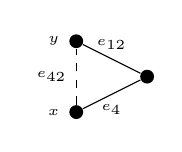
\begin{tikzpicture}[scale=0.3]
\tikzstyle{vertex}=[circle,fill=black,minimum size=5pt,inner sep=0pt]
\node[vertex, label=left:{\tiny $x$}] (0) at (0,0){};
\node[vertex, label=left:{\tiny $y$}] (1) at (0,3){};
\node[vertex] (2) at (3,1.5){};
\draw (2) -- (1)node[draw=none,fill=none,midway,above,font=\tiny] {$e_{12}$};
\draw (2) -- (0)node[draw=none,fill=none,midway,below,font=\tiny,] {$e_4$};
\draw[dashed] (0) -- (1)node[draw=none,fill=none,midway,left,font=\tiny,] {$e_{42}$};
\end{tikzpicture}
\end{center}
\end{minipage}
\begin{minipage}[t]{0.31\linewidth}
\vspace{0.5cm}
\begin{center}
\begin{tabular}{l|l}
\tiny{{x,y}} & \tiny{$est.1$}\\
\tiny{{c,d}} & \tiny{$est.3$}\\
\tiny{{u,v}} & \tiny{$est.12$}\\
  \end{tabular}
\end{center}
\end{minipage}
\begin{minipage}[t]{0.31\linewidth}
\vspace{0.5cm}
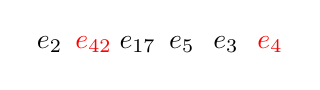
\begin{tikzpicture}[scale=0.8]
\tikzstyle{recti}=[rectangle,draw=red,thick,minimum width=3.3cm,minimum height=0.4cm]
\tikzstyle{stream}=[rectangle,]
\node [stream] at (6,0) {\color{red}$e_{4}$};
\node [stream] at (5.3,0) {{$e_3$}};
\node [stream] at (4.6,0) {{$e_5$}};
\node [stream] at (3.9,0) {$e_{17}$};
\node [stream] at (3.2,0) {\color{red}$e_{42}$};
\node [stream] at (2.5,0) {{$e_2$}};
\end{tikzpicture}
\end{minipage}
\end{frame}

\section{Sampling Triangles}
\begin{frame}

\end{frame}
\section{Experiments and Results}
\begin{frame}
\end{frame}
\section{Discussion}
\begin{frame}
\end{frame}
\end{document}
